\documentclass[m,binding,scrreprt,master,palatino]{WeSTthesis}
%\documentclass[m,binding,twoside,scrreprt,master,palatino]{WeSTthesis}
\usepackage[english,ngerman]{babel}		% English and new German spelling
\usepackage[utf8]{inputenc}           % correct input encoding
\usepackage[T1]{fontenc}              % correct output encoding
\usepackage{graphicx}					      	% enhanced support for graphics
\usepackage{tabularx}				      		% more flexible tabular
\usepackage{amsfonts}					      	% math fonts
\usepackage{amssymb}					      	%	math symbols
\usepackage{amsmath}					      	% overall enhancements to math environment
\usepackage[textsize=footnotesize,textwidth=27.5mm]{todonotes}					      	% package for notes/comments
\usepackage[bookmarks=true,
bookmarksopen=true,
bookmarksnumbered=true,
pdfstartpage=1,
%TODO add final title
pdftitle={},
pdfauthor={Martin Christian Körner},
pdfsubject={Master's Thesis},
%TODO add keywords
pdfkeywords={},
breaklinks=true,
colorlinks=true,
linkcolor=black,
anchorcolor=black,
citecolor=black,
filecolor=black,
menucolor=black,
urlcolor=black]{hyperref}
%\usepackage{hyperref}
\usepackage{float}                    % additional positions for images
\usepackage{listings}                 % source code
\usepackage[font=bf,labelfont=bf]{caption}    % captions
\usepackage{appendix}                 % appendix
\usepackage{microtype}
\usepackage{multirow}% http://ctan.org/pkg/multirow
\usepackage{epstopdf}
\usepackage{cleveref}

\newcommand{\itodo}[1]{\todo[inline]{#1}}

% Make cref auto-capitalize labels
\renewcommand{\cref}{\Cref}

%TODO add matriculation number to WeSTthesis.cls?
\author{Martin Körner\\[0.1cm]\normalsize{Matrikelnummer: 210200113}\vspace{-0.5cm}}

\title{Reference String Extraction from\\
Social Science Research Papers using\\
Conditional Random Fields and\\
Distant Supervision}

\degreecourse{Web Science}

\firstreviewer{Prof. Dr. Steffen Staab}
\firstreviewerinfo{Institute for Web Science and Technologies}

\secondreviewer{Ren\'e Pickhardt}
\secondreviewerinfo{Institute for Web Science and Technologies}

\begin{document}
\pagenumbering{roman}

\maketitle

\begin{center}
  \begin{large}
  \bfseries{Zusammenfassung}
  \end{large}
\end{center}
Zusammenfassung auf Deutsch
\par\bigskip
\par\bigskip
\selectlanguage{english}
\begin{center}
  \begin{large}
  \bfseries{Abstract}
  \end{large}
\end{center}
To help in overcoming a shortage of citation information for the German social sciences, we contribute an approach for extracting author names from reference sections.
Instead of relying on small amounts of manually labeled data, we use a distantly supervised approach to automatically generate a partially labeled training data set.
To apply this data set to the widely used probabilistic framework of conditional random fields, GE criteria provide a suitable objective function.
The resulting model does not only decide if a word is part of an author, but also separates the listed authors and distinguishes between first and last names.
The evaluation of our model reports a promising performance for the author extraction task.
In addition, it suggests ways of influencing the trade-off between the precision and recall of the model.

\varclearpage

%TODO add license
%\begin{center}
\includegraphics{figures/cc-by-sa.eps}
\end{center}
\begin{small}
This work is licensed under the Creative Commons Attribution-ShareAlike 4.0 International License. To view a copy of this license, visit \url{http://creativecommons.org/licenses/by-sa/4.0/}.
\end{small}

%\varclearpage

\tableofcontents
\varclearpage

\pagenumbering{arabic}
% list of figures
% \listoffigures
% \varclearpage

% beginning of the actual text section
%\listoftodos
\clearpage
\chapter{Introduction}\label{cha:introduction}

% What is the thesis about?
% Why is it relevant or important?
% What are the issues or problems?
% What is the proposed solution or approach?
% What can one expect in the rest of the thesis?


Citation data provides information on which scholarly work cites with other scholarly work.
This information is essential for the knowledge discovery process when conducting research and there are several services available that provide citation data for research areas like mathematics and physics\footnote{\url{http://related-work.net/}}, computer science\footnote{\url{http://dblp.uni-trier.de/}}, and medicine\footnote{\url{http://www.ncbi.nlm.nih.gov/pubmed}}.
Despite its importance, there is a shortage of citation data for German social science research papers~\cite{herb2015open}.
Even though there are commercial services available which provide citation data for a broad range of research areas, they do not provide a sufficient coverage of smaller academic fields like the German social sciences.
This could be explained by the low profitability of including such data.
In addition, commercial services generally do not publicly share their dataset which hinders a full utilization of the citation data.
The Social Science Citation Index\footnote{\url{http://scientific.thomson.com/products/ssci/}} by Thomson Reuters in particular was criticized for being ideologically biased and containing methodological deficiencies in the citation counting~\cite{klein2004social}.
Thereby, the motivation of this thesis is to contribute to the effort of extracting citation data from given research papers in order fill the gap regarding the German social sciences and to be less dependent on commercial services.

\bigskip

The different steps for extracting citation data from PDF documents are shown in \todo{add}.
At first the content of the PDF files is converted to text files to allow easier processing.
In the second step the reference strings are extracted from the text.
The strings are then segmented into the different attributes that identify the referenced paper (step three).

Such attributes can be the authors, title, journal, and publication year.
This information then needs to be matched against existing meta data records in order to assign a unique identifier such as a \gls{doi} to the reference (step four) to generate a citation network.
This thesis has not the goal of covering the whole pipeline.
Instead, we focus on the extraction reference strings from a given article in plain text.

\itodo{clarify/define reference vs citation}

The implementations that result from thesis are available on \todo{link} under a open-source license.


The remainder of this thesis is structured as follows.
In \Cref{cha:introduction} we introduce the problem of reference string extraction and in particular the extraction of author names in references.



\varclearpage

%\bibliographystyle{plain}
\bibliographystyle{alpha}

\bibliography{frontbackmatter/bibliography}
\varclearpage

%\appendix
%\appendixpage
%\addappheadtotoc
%\input{appendices/insert-filename-here}
%\varclearpage

\pagenumbering{gooble}
%\input{danksagung}
\end{document}
